% ============================================================================
% Chapter 4: System Design and Architecture
% ============================================================================

\chapter{System Design and Architecture}
\label{chap:design}

This chapter presents the comprehensive system design for the IntelliRoom platform, documenting the technical architecture, database schema, API design, and implementation details. The designs reflect the current implementation state with clear indication of completed and planned components.

% ============================================================================
\section{System Architecture Overview}
\label{sec:architecture}

The IntelliRoom platform follows a modern three-tier architecture with containerized deployment, separating concerns between frontend presentation, backend API services, AI processing pipelines, and data storage layers. Figure~\ref{fig:architecture} illustrates the high-level system architecture.

\begin{figure}[htbp]
    \centering
    \includegraphics[width=1\textwidth]{figures/system_architecture_tikz.pdf}
    \caption{High-Level System Architecture Diagram}
    \label{fig:architecture}
\end{figure}

\subsection{Architecture Layers}

The implemented architecture consists of the following layers:

\begin{enumerate}
    \item \textbf{Presentation Layer:} React.js-based web application with component-based architecture. The frontend implements responsive design principles and is structured with dedicated folders for components, screens, services, context, hooks, and utilities.
    
    \item \textbf{API Layer:} Node.js with Express framework serving RESTful endpoints on port 5000. The backend implements:
    \begin{itemize}
        \item CORS middleware for cross-origin request handling
        \item Static file serving for uploaded images and ComfyUI outputs
        \item Modular route organization by domain (ecommerce, design2D, upload)
    \end{itemize}
    
    \item \textbf{Service Layer:} Domain-specific services organized by functionality:
    \begin{itemize}
        \item \textbf{E-commerce Service:} Product catalog, shopping cart, orders, categories, wishlist management
        \item \textbf{Design 2D Service:} Project management, floor planning, 3D asset handling
        \item \textbf{Upload Service:} Image upload with ComfyUI processing integration
        \item \textbf{Authentication Service:} User registration (signup) implemented; login and token refresh flows planned and currently disabled in routes
        \item \textbf{Plugin Marketplace Service:} Community plugins with CRUD operations, ratings, and reviews
        \item \textbf{Contact Service:} Contact form submission handling
    \end{itemize}
    
    \item \textbf{AI Processing Layer:} Logic for managing generative AI workflows and model inference:
    \begin{itemize}
        \item \textbf{ComfyUI Engine:} Node-based engine executing complex generative workflows including Stable Diffusion, ControlNet, and SAM2.
        \item \textbf{Direct Integration:} The Node.js backend communicates directly with the ComfyUI API to trigger workflows and retrieve results.
        \item \textbf{AI Service Container:} A Python-based FastAPI service is scaffolded for future custom model serving.
    \end{itemize}
    
    \item \textbf{Data Layer:} MongoDB 7 document database with Mongoose ODM:
    \begin{itemize}
        \item \textbf{MongoDB:} Primary database for all structured data
        \item \textbf{File Storage:} Local storage for uploaded images and generated outputs
    \end{itemize}
\end{enumerate}

% ============================================================================
\section{Containerization and Deployment}
\label{sec:containerization}

The IntelliRoom platform utilizes Docker for containerized deployment, enabling consistent development environments and simplified deployment.

\subsection{Docker Compose Configuration}

The system is orchestrated using Docker Compose with the following services:

The Compose configuration defines a development container that runs the React frontend and Node.js backend with live source mounting and port exposure for both services. It depends on a MongoDB 7 database container that is configured with authentication, persistent storage, and a dedicated bridge network. A named volume is used to ensure database persistence across restarts.

\subsection{AI Service Container}

A separate Docker configuration handles the AI processing service:

The AI container definition is scaffolded with a lightweight Python runtime, system build tools, and project dependencies. The configuration targets a Uvicorn entrypoint on port 8000, but the FastAPI application module is not yet present in the repository. This service remains planned until the app entrypoint is implemented.

% ============================================================================
\section{Backend API Architecture}
\label{sec:backend_api}

The backend follows a modular MVC-like architecture with clear separation between routes, controllers, models, and services.

\subsection{Directory Structure}

The backend source code is organized as follows:

The backend is organized into configuration, controllers, middleware, models, routes, services, and a server entry point. Controllers are grouped by domain (Design 2D, E-commerce, Upload, Authentication, Plugins, and Contact), while models are split into design, commerce, user/community, credit/object, plugin, and contact collections. Service utilities handle integrations such as the ComfyUI connector.

\subsection{API Endpoints}

Table~\ref{tab:api_endpoints} documents the implemented REST API endpoints.

\begin{longtable}{|p{2cm}|p{4cm}|p{6.5cm}|}
    \caption{Implemented API Endpoints} \label{tab:api_endpoints} \\
    \hline
    \textbf{Method} & \textbf{Endpoint} & \textbf{Description} \\
    \hline
    \endfirsthead
    \hline
    \textbf{Method} & \textbf{Endpoint} & \textbf{Description} \\
    \hline
    \endhead
    \hline
    \endfoot
    
    \multicolumn{3}{|c|}{\textbf{E-commerce Routes (/api/ecommerce)}} \\
    \hline
    GET & /products & Get products with search, pagination, sorting \\
    \hline
    GET & /products/:id & Get single product by ID \\
    \hline
    POST & /products & Create new product \\
    \hline
    PUT & /products/:id & Update product \\
    \hline
    DELETE & /products/:id & Delete product \\
    \hline
    GET & /categories & Get all categories \\
    \hline
    POST & /categories & Create category \\
    \hline
    GET & /cart & Get user's shopping cart \\
    \hline
    POST & /cart & Create new cart \\
    \hline
    PUT & /cart/:id & Update cart items \\
    \hline
    DELETE & /cart/:id & Delete cart \\
    \hline
    GET & /wishlist & Get user's wishlist \\
    \hline
    POST & /wishlist & Add item to wishlist \\
    \hline
    DELETE & /wishlist/:id & Remove from wishlist \\
    \hline
    GET & /order & Get user's orders \\
    \hline
    POST & /order & Create new order \\
    \hline
    \multicolumn{3}{|c|}{\textbf{Design 2D Routes (/api/design2D)}} \\
    \hline
    GET & /projects & Get all user projects \\
    \hline
    GET & /projects/:id & Get project by ID \\
    \hline
    POST & /projects & Create new project \\
    \hline
    PUT & /projects/:id & Update project \\
    \hline
    DELETE & /projects/:id & Delete project \\
    \hline
    GET & /assets & Get available 3D assets \\
    \hline
    \multicolumn{3}{|c|}{\textbf{Upload Routes (/api/uploadImage)}} \\
    \hline
    POST & / & Upload image for AI processing \\
    \hline
    \multicolumn{3}{|c|}{\textbf{Authentication Routes}} \\
    \hline
    POST & /api/auth/login & User login (currently disabled in code) \\
    \hline
    POST & /api/signup & User registration with username, email, password \\
    \hline
    \multicolumn{3}{|c|}{\textbf{Plugin Marketplace Routes (/api/plugins)}} \\
    \hline
    GET & / & Get all plugins with author info \\
    \hline
    GET & /:id & Get plugin details by ID \\
    \hline
    POST & / & Create new plugin \\
    \hline
    PUT & /:id & Update plugin (author-only) \\
    \hline
    DELETE & /:id & Delete plugin (author-only) \\
    \hline
    \multicolumn{3}{|c|}{\textbf{Contact Routes (/api/contact)}} \\
    \hline
    POST & / & Submit contact form message \\
    \hline
\end{longtable}

\subsection{Server Configuration}

The main server entry point configures Express with middleware and route mounting:

The server initializes environment variables, connects to MongoDB, enables JSON parsing and CORS, and exposes static directories for uploaded images and generated outputs at \texttt{/api/uploads} and \texttt{/api/comfyOutputs}. It mounts domain routes for e-commerce, design, and uploads, then starts listening on a configurable port. The ComfyUI integration is instantiated during startup using a configurable host address.

% ============================================================================
\section{Database Design}
\label{sec:database}

The IntelliRoom platform employs MongoDB as its primary database, selected for its flexible document model, horizontal scalability, and native JSON support that aligns naturally with the JavaScript/Node.js backend stack. The database architecture is organized into two logical domains reflecting the platform's modular structure: Core \& Commerce operations and Design \& Community features.

\subsection{Database Architecture Rationale}

\subsubsection{Why MongoDB?}

Several factors influenced the selection of MongoDB over relational databases:

\begin{enumerate}
    \item \textbf{Schema Flexibility:} The \texttt{sceneData} field in Project documents stores complex 2D/3D scene hierarchies with varying structures. MongoDB's document model accommodates this variability without rigid table schemas.
    
    \item \textbf{Developer Productivity:} Mongoose ODM provides TypeScript-like schema validation while maintaining MongoDB's flexibility, enabling rapid iteration during development.
    
    \item \textbf{Scalability:} Built-in sharding and replica sets support horizontal scaling as user base grows beyond initial Egyptian market.
    
    \item \textbf{JSON-Native:} Direct JSON storage eliminates ORM impedance mismatch, particularly beneficial for REST APIs returning JSON responses.
\end{enumerate}

\subsubsection{Document vs. Relational Design Decisions}

The schema employs a hybrid approach combining embedded documents and references:

\begin{itemize}
    \item \textbf{Embedded Documents:} \texttt{CartItem} and \texttt{OrderItem} are embedded within their parent documents (Cart, Order) since they have no independent lifecycle and are always accessed with their parent.
    
    \item \textbf{References:} User, Product, and Category maintain separate collections with ObjectId references, enabling independent queries and updates without duplication.
    
    \item \textbf{Denormalization:} Product name and price are duplicated in OrderItem to preserve historical order data even if product details change later.
\end{itemize}

\subsection{Entity-Relationship Overview}

The database schema is organized into two primary domains: (1) Core User and E-commerce entities, and (2) Design and Community entities. This separation reflects the modular architecture of the platform while maintaining the User entity as the central linking point across both domains.

\subsubsection{Core \& Commerce Schema}

Figure~\ref{fig:erd_core} presents the core user management and e-commerce entities. The schema centers on the \textbf{User} entity, which serves as the authentication and authorization anchor for the entire system.

\begin{figure}[htbp]
    \centering
    \includegraphics[width=1.0\textwidth]{figures/erd_core_commerce.pdf}
    \caption{Core \& Commerce Schema: User, Credits, Cart, Order, Product, Category}
    \label{fig:erd_core}
\end{figure}

\textbf{Key Relationships in Core \& Commerce Schema:}

\begin{itemize}
    \item \textbf{User $\rightarrow$ CreditTransaction (1:N):} Each user accumulates a history of credit transactions (spent/earned), enabling audit trails and usage analytics. The separate collection supports efficient querying of transaction history without loading full user documents.
    
    \item \textbf{User $\rightarrow$ Cart (1:1):} Each user maintains a single persistent shopping cart. The cart stores a reference to the user and contains an embedded array of CartItem subdocuments.
    
    \item \textbf{Cart $\rightarrow$ CartItem (1:N, Embedded):} CartItems are embedded within the Cart document. Each item references a Product and stores the quantity and price at time of addition (preserving price if product pricing changes).
    
    \item \textbf{User $\rightarrow$ Order (1:N):} Users can place multiple orders over time. Orders are separate documents to support independent querying, status updates, and historical analysis.
    
    \item \textbf{Order $\rightarrow$ OrderItem (1:N, Embedded):} OrderItems are embedded within Order documents, capturing product name, price, quantity, and image at purchase time. This denormalization ensures order history remains accurate even if products are modified or deleted.
    
    \item \textbf{CartItem/OrderItem $\rightarrow$ Product (M:1):} Both cart and order items reference Product documents via ObjectId. This maintains data integrity while allowing product updates without affecting existing carts/orders (due to denormalized fields).
    
    \item \textbf{Product $\rightarrow$ Category (N:1):} Products belong to a single category (e.g., "Living Room Furniture", "Bedroom Furniture"). Categories enable faceted search and filtering in the marketplace.
\end{itemize}

\textbf{Design Decisions:}

\begin{itemize}
    \item The \texttt{plan} field in User stores subscription tier (free, monthly, yearly) as an enum, enabling feature gating and usage limit enforcement.
    \item The \texttt{credits} field tracks remaining balance, updated atomically via MongoDB \texttt{\$inc} operator to prevent race conditions.
    \item Cart persistence across sessions reduces friction in the purchasing funnel, addressing the high cart abandonment rates (90\%+) documented in the Egyptian e-commerce market.
\end{itemize}

\subsubsection{Design \& Community Schema}

Figure~\ref{fig:erd_design} illustrates the design workflow and community features. This schema centers on the creative pipeline from Project creation through AI generation to community sharing.

\begin{figure}[htbp]
    \centering
    \includegraphics[width=1.0\textwidth]{figures/erd_design_community.pdf}
    \caption{Design \& Community Schema: Project, 2D/3D Design, Style, Assets, Gallery}
    \label{fig:erd_design}
\end{figure}

\textbf{Key Relationships in Design \& Community Schema:}

\begin{itemize}
    \item \textbf{User $\rightarrow$ Project (1:N):} Users create multiple design projects. Each project stores flexible \texttt{sceneData} as a JSON object, accommodating various 2D/3D scene structures without schema migrations.
    
    \item \textbf{Project $\rightarrow$ 2D Design (1:N):} A project can contain multiple 2D design iterations. The \texttt{version} field in Project enables tracking design evolution.
    
    \item \textbf{2D Design $\rightarrow$ 3D Design (1:N):} Each 2D design can be expanded into multiple 3D representations. The \texttt{is\_public} flag controls whether designs appear in the community gallery.
    
    \item \textbf{Style $\rightarrow$ 2D Design (1:N):} Styles represent reusable design templates (e.g., "Modern Egyptian", "Arabic Traditional"). The \texttt{config\_data} field stores AI model parameters (LoRA weights, ControlNet settings) required for style application.
    
    \item \textbf{3D Design $\rightarrow$ Object (1:N):} 3D designs reference multiple Object entities representing furniture and decor items. Objects include \texttt{object\_model\_url} for 3D mesh files and \texttt{provider} for e-commerce integration.
    
    \item \textbf{User $\rightarrow$ GalleryPost (1:N):} Users share designs publicly via gallery posts. Each post includes \texttt{likes}, \texttt{tags}, and an optional \texttt{caption} for community engagement.
    
    \item \textbf{2D Design $\rightarrow$ GalleryPost (1:N):} A design can be featured in multiple gallery posts (e.g., before/after comparisons, different room angles).
    
    \item \textbf{User $\rightarrow$ Comment (1:N):} Users comment on gallery posts. Comments are stored as separate documents to support pagination and moderation workflows.
    
    \item \textbf{User $\rightarrow$ Reaction (1:N):} The Reaction entity supports likes, upvotes, and downvotes on both posts and comments. The \texttt{target\_type} field enables polymorphic associations.
\end{itemize}

\textbf{Design Decisions:}

\begin{itemize}
    \item The \texttt{sceneData} field in Project uses MongoDB's flexible schema to store varying scene structures (2D floor plans, 3D scenes, mixed layouts) without requiring schema migrations as features evolve.
    
    \item The \texttt{Style} entity separates design aesthetics from project data, enabling users to apply community-created styles to their designs. The \texttt{config\_data} field stores AI parameters in JSON format.
    
    \item \texttt{FloorPlanObject} and \texttt{Assets} entities maintain catalogs of reusable 3D assets with metadata (dimensions, categories, constraints) for drag-and-drop functionality in the 2D/3D planner.
    
    \item Gallery posts decouple social features from design storage, allowing users to share designs without exposing full project data. The \texttt{tags} array enables content discovery and trending topic tracking.
\end{itemize}

\subsection{Schema Definitions}

\subsubsection{User Schema}

The User schema stores account information, subscription plans, and credit balance:

Key fields include a unique user identifier, username, email, hashed password, profile data, credit balance, and subscription plan. Timestamps are recorded for account creation and updates. A first-time flag supports onboarding logic, and the wishlist stores product references.

\subsubsection{Project Schema (2D/3D Design)}

The Project schema stores design projects with flexible sceneData for 2D/3D scenes:

Each project references its owner, includes a title and version, and stores full 2D/3D scene data as a flexible structure. Optional cover and thumbnail images support previews, while timestamps capture creation and update times.

\subsubsection{Product Schema (E-commerce)}

The Product schema supports the furniture marketplace:

Product records include name, description, price, category reference, inventory stock, and a list of image URLs with optional alt text. Review data is captured via rating and review count, while a featured flag supports merchandising. Timestamps are enabled for auditing.

\subsubsection{Gallery Post Schema (Community)}

The GalleryPost schema enables community sharing:

Community posts store a unique post identifier, user reference, optional design reference, post text, like counts, and tags. Comments are embedded with user identifiers, text, and timestamps. Each post maintains creation and update timestamps for moderation workflows.

\subsubsection{Credit Transaction Schema}

The CreditTransaction schema tracks credit usage:

Each credit transaction records a unique identifier, amount, and transaction type (spent or earned). A timestamp and descriptive note are stored for each transaction. The collection is stored separately and does not use automatic timestamps.

\subsubsection{3D Object Schema}

The Object schema stores 3D furniture assets for the floor planner:

3D asset records include a unique identifier, object name and type, preview image URL, model file URL, default color, configuration metadata, and the associated e-commerce provider. Timestamping is enabled for catalog tracking.

\subsubsection{Plugin Schema (Community Marketplace)}

The Plugin schema enables the community plugin marketplace:

Each plugin record stores a unique identifier, plugin name, description, author reference (linked to User), rating, reviews array, included features list, download count, and pricing in credits. Timestamps track creation and updates, enabling plugin discovery by recency.

\subsubsection{Contact Schema}

The Contact schema stores contact form submissions:

Contact records capture the sender's name, email, subject line, and message body. Automatic timestamps enable follow-up tracking and support queue management.

% ============================================================================
\section{ComfyUI Integration Service}
\label{sec:comfyui}

The ComfyUI integration represents a key technical component enabling AI-powered image processing. The service implements REST API polling for workflow status monitoring.

\subsection{Service Architecture}

The ComfyUIService class provides the following capabilities:

\begin{enumerate}
    \item \textbf{REST API Polling:} HTTP-based status polling to ComfyUI server for workflow monitoring
    \item \textbf{Image Upload:} Upload images to ComfyUI input directory for processing
    \item \textbf{Workflow Execution:} Submit and track node-based AI workflows
    \item \textbf{Completion Polling:} Periodic status checks until workflow history is available
    \item \textbf{Result Retrieval:} Download processed images from ComfyUI output
    \item \textbf{Zrok Support:} Compatibility with zrok tunneling for remote ComfyUI access
\end{enumerate}

\subsection{ComfyUI Service Implementation}

The service uses HTTP polling to track workflow execution status:

The service polls the ComfyUI server's history endpoint at regular intervals to check workflow completion status. It resolves a job once the workflow history contains outputs. A five-minute timeout protects the system from stalled executions. For remote access via zrok, the client adds a custom header to bypass the interstitial screen.

\subsection{Image Upload and Workflow Execution}

The service provides methods for uploading images and running workflows:

Image uploads are sent to the ComfyUI upload endpoint with optional subfolder placement. Workflow execution is requested through the prompt endpoint, after which the service polls history until outputs are available. A five-minute timeout protects the system from stalled executions.

\subsection{Sample Workflow Definition}

The repository includes ComfyUI workflow definitions that are imported and executed by the ComfyUI engine. These workflow files serve as the reference implementations for generation tasks and can be executed directly in ComfyUI.

% ============================================================================
\section{AI Pipeline Architecture}
\label{sec:ai_pipeline}

The planned AI generation pipeline will leverage the ComfyUI infrastructure with advanced models for interior design transformation.

\subsection{Planned Pipeline Stages}

\begin{enumerate}
    \item \textbf{Input Processing:} Room photograph upload, validation, and preprocessing
    \item \textbf{Object Detection:} Florence-2 model for room type and furniture identification
    \item \textbf{Semantic Segmentation:} SAM2 for precise furniture and room element masks
    \item \textbf{Style Configuration:} User-selected cultural style presets (Arabic, Egyptian)
    \item \textbf{Generative Transformation:} ControlNet-guided style transfer with structure preservation
    \item \textbf{Compositing:} Seamless blending and quality enhancement
    \item \textbf{Output Generation:} Multiple design variations with furniture recommendations
\end{enumerate}

\subsection{AI Service Dependencies}

The Python-based AI service includes the following dependencies:

The AI service dependencies are declared in \texttt{ai/requirements.txt}, including FastAPI (0.115.4) and Uvicorn (0.32.0) for the API layer, PyTorch (2.5.1) and Transformers (4.45.2) for model execution, and data utilities such as Pandas (2.2.3), NumPy (2.1.2), and scikit-learn (1.5.2). Validation and async support rely on Pydantic (2.9.2), Starlette (0.41.2), and HTTPX (0.27.2). The service entrypoint remains planned until the FastAPI app module is implemented.

\subsection{Single-View 3D Object Reconstruction Pipeline}
\label{subsec:3d_reconstruction}

To bridge the gap between 2D inspiration and 3D spatial planning, IntelliRoom incorporates a dedicated pipeline for Single-View 3D Reconstruction. This module allows users to upload a single photograph of a furniture piece (e.g., a heritage chair or a specific marketplace find) and converts it into a textured 3D mesh (.GLB format) suitable for AR visualization or CAD integration.

The pipeline utilizes the Hunyuan3D-2.0 architecture, orchestrated via ComfyUI. Unlike traditional photogrammetry which requires dozens of overlapping images, this generative approach infers 3D geometry from a single viewpoint using a two-stage process.

\begin{figure}[htbp]
    \centering
    \includegraphics[width=1.0\textwidth]{figures/wf_Part1.png}
    \caption{3D Reconstruction Pipeline Part 1: Initial image loading, segmentation (InSpyReNet), and geometry generation via Hunyuan3D DiT.}
    \label{fig:3d_workflow_part1}
\end{figure}

\subsubsection*{Stage 1: Preprocessing and Segmentation}

The input image first undergoes rigorous preprocessing to ensure clean geometry generation:

\begin{itemize}
    \item \textbf{Background Removal:} The system employs InSpyReNet, a high-fidelity segmentation model, to remove the background and isolate the subject. This prevents background noise (e.g., floor tiles, shadows) from being interpreted as physical geometry.
    \item \textbf{Normalization:} The segmented image is resized (typically to $512 \times 512$) and centered to align with the training distribution of the diffusion model.
\end{itemize}

\subsubsection*{Stage 2: Geometry Generation (DiT)}

The core 3D shape is generated using a Diffusion Transformer (DiT) model (hunyuan3d-dit-v2-0).

\begin{itemize}
    \item \textbf{Latent Generation:} The model predicts a 3D implicit representation (Signed Distance Field - SDF) in latent space based on the 2D visual conditioning.
    \item \textbf{Marching Cubes Decoding:} A VAE Decoder converts the latent representation into a raw mesh using the Marching Cubes algorithm.
    \item \textbf{Mesh Cleaning:} A post-processing node removes ``floaters'' (disconnected geometry artifacts) and degenerate faces to simplify the mesh for web rendering.
\end{itemize}

\begin{figure}[htbp]
    \centering
    \includegraphics[width=1.0\textwidth]{figures/wf_part2.png}
    \caption{3D Reconstruction Pipeline Part 2: Texture generation, delighting, and multi-view synthesis.}
    \label{fig:3d_workflow_part2}
\end{figure}

\subsubsection*{Stage 3: Texture Synthesis and Delighting}

Once the geometry is established, the pipeline applies high-fidelity textures:

\begin{itemize}
    \item \textbf{Delighting:} A Hy3D Delight module analyzes the original image to remove baked-in lighting information (shadows and highlights). This results in an ``Albedo'' map, allowing the 3D object to react naturally to new lighting environments in the 3D viewer.
    \item \textbf{Multi-View Painting:} The system uses a specialized paint model (hunyuan3d-paint-v2) to hallucinate the ``unseen'' sides of the object (e.g., the back of the chair) based on the style of the front view.
    \item \textbf{UV Mapping \& Inpainting:} The generated views are projected onto the mesh UVs. A CV2-based inpainting step fills any remaining texture gaps or seams.
\end{itemize}

\begin{figure}[htbp]
    \centering
    \includegraphics[width=1.0\textwidth]{figures/wf_part3.png}
    \caption{3D Reconstruction Pipeline Part 3: UV mapping, inpainting, upscaling, and final .GLB export.}
    \label{fig:3d_workflow_part3}
\end{figure}

\subsubsection*{Stage 4: Upscaling and Export}

To ensure visual fidelity, the texture maps are upscaled (to $2048 \times 2048$) before being baked onto the mesh. The final object is exported as a .GLB (glTF binary) file, which is optimized for web-based rendering in the IntelliRoom frontend.

\subsubsection*{Summary: From Pixel to Polygon}

\begin{itemize}
    \item \textbf{The Challenge:} Users want to see their specific furniture in the room, not generic 3D models.
    \item \textbf{The Solution:} Single-Image-to-3D Pipeline using Hunyuan3D 2.0.
    \item \textbf{The Process:}
    \begin{itemize}
        \item \textbf{Isolate:} AI removes background (InSpyReNet).
        \item \textbf{Sculpt:} Diffusion Transformer creates the 3D shape.
        \item \textbf{Paint:} AI hallucinates the ``back'' of the object and removes static shadows (Delighting).
    \end{itemize}
    \item \textbf{The Result:} A downloadable 3D .GLB file generated in under 45 seconds.
\end{itemize}

% ============================================================================
\section{ComfyUI Workflow Catalog}
\label{sec:comfyui_workflows}

This section documents the primary ComfyUI workflows that operationalize IntelliRoom's AI capabilities. Each workflow is designed as a modular pipeline that can be called independently or routed through the Universal Master Workflow described at the end of this section.

% ---------------------------------------------------------------------------
\subsection{Empty Room Furnishing Workflow}
\label{subsec:empty_room_workflow}

The Empty Room workflow addresses the requirement of furnishing an unfurnished space while preserving architectural structure. It operates as an image-to-image (img2img) pipeline guided by a CR Multi-ControlNet stack to maintain walls, windows, and perspective fidelity.

\begin{figure}[htbp]
    \centering
    \includegraphics[width=1.0\textwidth]{figures/emptyroom_workflow_dark.png}
    \caption{Empty Room Furnishing Workflow: Multi-ControlNet guided img2img pipeline preserving architectural structure while generating furniture.}
    \label{fig:emptyroom_workflow}
\end{figure}

\subsubsection*{Workflow Architecture}

\textbf{Input and Conditioning}
\begin{itemize}
    \item \textbf{Checkpoint:} RealisticVisionV6 (photorealistic interiors).
    \item \textbf{Input:} User-provided empty room image (Load Image node).
    \item \textbf{Prompting:} Simple positive prompts (e.g., ``living room'') and strict negative prompts (e.g., ``text'') to reduce artifacts.
\end{itemize}

\textbf{Multi-ControlNet Stacking}
\begin{itemize}
    \item \textbf{Canny Edge (Strength 1.00):} Locks high-frequency architectural details (windows, fixtures).
    \item \textbf{M-LSD (Strength 0.40):} Preserves straight lines and perspective of walls and ceilings.
    \item \textbf{Depth (Off):} Disabled in the referenced snapshot when edge and line signals are sufficient.
\end{itemize}

\textbf{Latent Generation}
\begin{itemize}
    \item \textbf{KSampler:} dpmpp\_sde with karras scheduler, 12 steps, CFG 2.0.
    \item \textbf{Denoise:} 0.86 to allow furniture hallucination while retaining structure.
\end{itemize}

\textbf{Output}
\begin{itemize}
    \item VAE decode followed by Image Comparer for before/after validation.
\end{itemize}

\textbf{Integration with Requirements:} Supports FR-15 (structural preservation during style transformations).

% ---------------------------------------------------------------------------
\subsection{Object Replacement Workflow}
\label{subsec:object_replacement_workflow}

This workflow enables selective regeneration of furniture items without altering the rest of the room, using Florence-2 for detection and SAM2 for precision masks.

\begin{figure}[htbp]
    \centering
    \includegraphics[width=1.0\textwidth]{figures/object_replace_workflow.png}
    \caption{Object Replacement Workflow: Florence-2 detection and SAM2 segmentation enable precision inpainting of specific furniture items.}
    \label{fig:object_replace_workflow}
\end{figure}

\subsubsection*{Workflow Architecture}

\textbf{Intelligent Detection (Florence-2)}
\begin{itemize}
    \item Text-based detection (e.g., ``carpet'') produces bounding boxes for target objects.
\end{itemize}

\textbf{Precision Segmentation (SAM2)}
\begin{itemize}
    \item Generates pixel-level masks from Florence-2 boxes to isolate objects cleanly from background.
\end{itemize}

\textbf{Inpainting and Generation}
\begin{itemize}
    \item \textbf{Inpaint Crop:} Crops to masked region to maximize resolution.
    \item \textbf{ControlNet:} Inpaint preprocessor + Canny edge to preserve surrounding geometry.
    \item \textbf{KSampler:} Denoise 1.00 for complete replacement of target pixels.
\end{itemize}

% ---------------------------------------------------------------------------
\subsection{Object Replacement with Style Transfer}
\label{subsec:object_replacement_style_transfer}

This workflow extends selective replacement by injecting a reference product image, enabling realistic ``Shop This Look'' previews.

\begin{figure}[htbp]
    \centering
    \includegraphics[width=1.0\textwidth]{figures/object_replace_withStyleTransfer_workflow.png}
    \caption{Object Replacement with Style Transfer: IPAdapter injects reference product textures into the inpainting process for ``Shop This Look'' visualization.}
    \label{fig:object_replace_style_workflow}
\end{figure}

\subsubsection*{Workflow Architecture}

\textbf{Reference Image Loading}
\begin{itemize}
    \item Secondary reference image (e.g., a specific rug) is provided to guide texture and pattern synthesis.
\end{itemize}

\textbf{IPAdapter Injection}
\begin{itemize}
    \item IPAdapter Advanced encodes reference features and injects them into diffusion.
    \item Weight is set to 1.00 (linear) to closely mimic target patterns.
\end{itemize}

\textbf{Structure-Aware Synthesis}
\begin{itemize}
    \item Florence-2 + SAM2 provide masks; ControlNet ensures perspective consistency.
    \item KSampler denoise at 0.95 balances texture transfer and spatial fidelity.
\end{itemize}

\textbf{Integration with Requirements:} Supports FR-16 (selective replacement) and FR-22 (marketplace visualization).

% ---------------------------------------------------------------------------
\subsection{Sketch-to-Render Workflow}
\label{subsec:sketch_to_render_workflow}

This workflow converts sketches or CAD wireframes into photorealistic renders, accelerating professional concept visualization.

\begin{figure}[htbp]
    \centering
    \includegraphics[width=1.0\textwidth]{figures/sketch_workflow_dark.png}
    \caption{Sketch-to-Render Workflow: Tri-layer ControlNet stack (M-LSD, Lineart, DepthAnything) converts CAD wireframes into photorealistic renders.}
    \label{fig:sketch_workflow}
\end{figure}

\subsubsection*{Workflow Architecture}

\textbf{Input and Resolution Management}
\begin{itemize}
    \item Sketch input via Load Image node.
    \item SDXL Resolution Calculator determines optimal sampling dimensions.
\end{itemize}

\textbf{Tri-Layer ControlNet Stack}
\begin{itemize}
    \item \textbf{M-LSD (0.85):} Preserves perspective and straight lines.
    \item \textbf{Lineart (1.00):} Enforces drawing strokes and designer intent.
    \item \textbf{DepthAnythingV2 (1.00):} Provides volumetric depth cues.
\end{itemize}

\textbf{High-Fidelity Generation}
\begin{itemize}
    \item KSampler denoise 1.00 with 40 steps (dpmpp\_sde + karras) for full synthesis.
\end{itemize}

\textbf{Integration with Professional Requirements:} Supports rapid prototyping for the Professional Designer segment.

% ---------------------------------------------------------------------------
\subsection{Ultimate Upscale Workflow}
\label{subsec:ultimate_upscale_workflow}

The upscale workflow generates high-resolution outputs for premium exports (FR-30), using tiled diffusion to avoid VRAM constraints.

\begin{figure}[htbp]
    \centering
    \includegraphics[width=1.0\textwidth]{figures/UltimateUpScale_workflow.png}
    \caption{Ultimate Upscale Workflow: Tiled diffusion with 4x\_foolhardy\_Remacri upscaler and Tile ControlNet for high-resolution exports.}
    \label{fig:ultimate_upscale_workflow}
\end{figure}

\subsubsection*{Workflow Architecture}

\begin{itemize}
    \item \textbf{Upscaler:} 4x\_foolhardy\_Remacri.pth with scale factor 2.0.
    \item \textbf{Tile ControlNet:} SDXL union controlnet at strength 1.00 (SD 1.5 uses tile\_resample).
    \item \textbf{Denoise:} 0.37 to add detail without altering composition.
    \item \textbf{Seam Fix:} Internal tiling seam correction (denoise 1.00, width 64).
\end{itemize}

% ---------------------------------------------------------------------------
\subsection{Universal Master Workflow}
\label{subsec:universal_master_workflow}

The Universal Workflow consolidates all ComfyUI capabilities into a single logic-driven super-graph, enabling dynamic routing between modes without reloading separate JSON files. This ``One-Graph-to-Rule-Them-All'' approach allows the backend to switch between Empty Room, Object Replacement, Style Transfer, and Upscale modes instantly by toggling boolean control signals.

\begin{figure}[htbp]
    \centering
    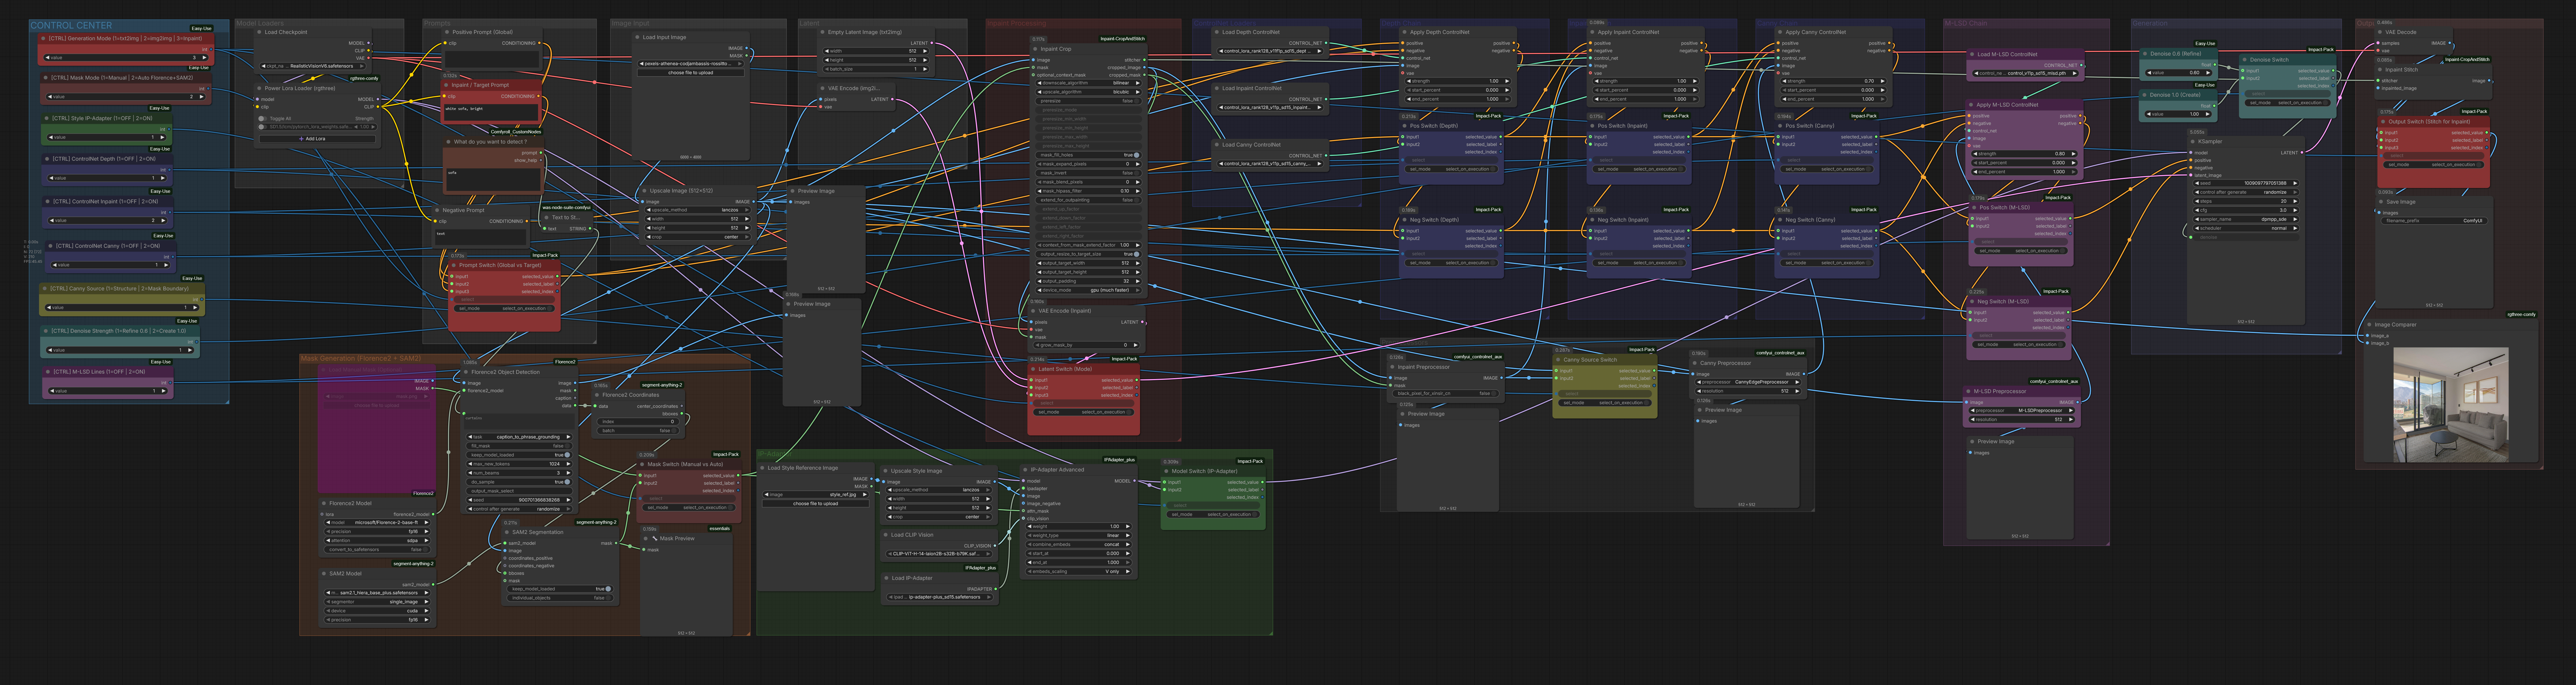
\includegraphics[width=1.0\textwidth]{figures/Universal_workflow_full_view.png}
    \caption{Universal Master Workflow: Complete node graph showing the Rail-Switch architecture that unifies all generation modes into a single configurable pipeline.}
    \label{fig:universal_workflow_full}
\end{figure}

The following subsections detail each functional block of the Universal Workflow, with zoomed views for clarity.

% - - - - - - - - - - - - - - - - - - - - - - - - - - - - - - - - - - - - - -
\subsubsection{Control Center and Input Logic}
\label{subsubsec:universal_control_center}

The Control Center, located on the far left of the workflow, acts as the pipeline's ``BIOS.'' A vertical stack of boolean switches controls the active state of the entire pipeline:

\begin{figure}[htbp]
    \centering
    \includegraphics[width=0.95\textwidth]{figures/Universal_workflow_view1.png}
    \caption{Control Center: Boolean switches (CTR1--CTR5) configure pipeline behavior without reloading the workflow.}
    \label{fig:universal_control_center}
\end{figure}

\begin{itemize}
    \item \textbf{[CTR1] Resize Source:} Toggles input image resizing logic.
    \item \textbf{[CTR2] Masking Mode:} Activates the specific style transfer logic path.
    \item \textbf{[CTR3] IP-Adapter:} Toggles reference image injection for ``Shop This Look'' functionality.
    \item \textbf{[CTR4] Controller Layer (In-Off):} Enables or disables specific ControlNet layers.
    \item \textbf{[CTR5] Invert Mask:} Toggles inpainting logic (preserve object vs. preserve background).
\end{itemize}

The Rail-Switch technique routes image data along a ``rail'' with boolean signals running in parallel. When a Control Center switch is set to \texttt{False}, the corresponding processing block is muted or bypassed entirely using ``Fast Muter'' and ``Any Switch'' nodes.

% - - - - - - - - - - - - - - - - - - - - - - - - - - - - - - - - - - - - - -
\subsubsection{Dynamic Segmentation Block}
\label{subsubsec:universal_segmentation}

When Florence-2 detection is enabled, the image is routed into the segmentation cluster for text-based object detection and mask generation.

\begin{figure}[htbp]
    \centering
    \includegraphics[width=0.95\textwidth]{figures/Universal_workflow_view2.png}
    \caption{Dynamic Segmentation Block: Florence-2 performs text-based detection (e.g., ``carpet'') and SAM2 generates pixel-level masks.}
    \label{fig:universal_segmentation}
\end{figure}

\begin{itemize}
    \item \textbf{Florence-2:} Receives text input and produces bounding box coordinates for target objects.
    \item \textbf{SAM2:} Takes bounding boxes and generates high-precision pixel masks.
    \item \textbf{Conditional Bypass:} If the segmentation switch is inactive (e.g., for Empty Room mode), this entire computational block is skipped, saving processing time.
\end{itemize}

% - - - - - - - - - - - - - - - - - - - - - - - - - - - - - - - - - - - - - -
\subsubsection{Conditioning Stack}
\label{subsubsec:universal_conditioning}

The central ``Rail'' manages the ControlNet stack, dynamically selecting which preprocessors and control signals are active based on the current mode.

\begin{figure}[htbp]
    \centering
    \includegraphics[width=0.95\textwidth]{figures/Universal_workflow_view3.png}
    \caption{Conditioning Stack: Logic gates dynamically swap between Canny (structure), Depth (volume), or M-LSD (lines) based on CTR settings.}
    \label{fig:universal_conditioning}
\end{figure}

Unlike the static Empty Room workflow with fixed ControlNets, the Universal Workflow uses logic gates to:
\begin{itemize}
    \item Select appropriate preprocessors (Canny Edge, M-LSD, DepthAnything) based on mode.
    \item Adjust ControlNet strengths dynamically.
    \item Route structural guidance signals to the generation phase.
\end{itemize}

% - - - - - - - - - - - - - - - - - - - - - - - - - - - - - - - - - - - - - -
\subsubsection{Style Injection Block}
\label{subsubsec:universal_style_injection}

This block houses the IPAdapter logic for reference-based style transfer, enabling users to visualize specific marketplace products in their rooms.

\begin{figure}[htbp]
    \centering
    \includegraphics[width=0.95\textwidth]{figures/Universal_workflow_view4.png}
    \caption{Style Injection Block: IPAdapter encodes reference product features and injects them into the diffusion latent space.}
    \label{fig:universal_style_injection}
\end{figure}

\begin{itemize}
    \item \textbf{Style Switch:} When the user uploads a reference image (e.g., a specific rug pattern), the switch closes and injects the style into the latent space.
    \item \textbf{No Reference Fallback:} If no reference is provided, the switch opens and the model relies solely on the text prompt.
    \item \textbf{Weight Configuration:} IPAdapter weight is typically set to 1.00 (linear) for close pattern matching.
\end{itemize}

% - - - - - - - - - - - - - - - - - - - - - - - - - - - - - - - - - - - - - -
\subsubsection{Unified Generation and Output}
\label{subsubsec:universal_generation}

Regardless of the path taken (segmentation, conditioning, or style injection), all data converges at a unified KSampler for final generation.

\begin{figure}[htbp]
    \centering
    \includegraphics[width=0.95\textwidth]{figures/Universal_workflow_view5.png}
    \caption{Unified Generation and Output: Single KSampler path with optional routing to Ultimate SD Upscale for 4K refinement.}
    \label{fig:universal_generation}
\end{figure}

\begin{itemize}
    \item \textbf{KSampler:} Central generation node receiving all conditioning signals.
    \item \textbf{Output Routing:} A final switch determines whether the image is saved immediately or sent to the Ultimate SD Upscale loop for high-resolution export.
    \item \textbf{VAE Decode:} Converts latent representation to final RGB image.
\end{itemize}

\subsubsection*{Strategic Value}

The Universal Workflow satisfies Non-Functional Requirement NFR-01 (Performance) by eliminating workflow reload latency, and NFR-13 (Maintainability) by centralizing model updates. When the team upgrades the underlying checkpoint (e.g., swapping RealisticVisionV6 for a newer model), the improvement instantly propagates to Empty Room, Replacement, Sketch, and Upscale modes simultaneously.

% ============================================================================
\newpage
\section{Frontend Architecture}
\label{sec:frontend}

The frontend application uses React.js with a component-based architecture and React Router for navigation.

\subsection{Directory Structure}

The frontend codebase is structured into reusable components, context providers, and custom hooks. It also includes page-level screens, API service modules, shared styles, and utility helpers. The application entry point (App.jsx) initializes the React application and mounts the Routes component.

\subsection{Implemented Screens}

The following screens have been implemented:

\begin{itemize}
    \item \textbf{Plugin Marketplace:} Community marketplace for custom styles and plugins, featuring:
    \begin{itemize}
        \item Search and filter functionality (by most recent, highest rated, most downloaded, price)
        \item Category browsing (Style Presets, Custom Configs, AI Plugins, Community Bundles)
        \item Plugin cards displaying title, author, rating, reviews, and pricing
        \item Featured and trending sections
        \item Loading and error states
        \item Responsive grid layout
    \end{itemize}
\end{itemize}

\subsection{Component Architecture}

The frontend implements a modular component architecture:

\begin{itemize}
    \item \textbf{Common Components:} Reusable UI elements including Header and Footer
    \item \textbf{Plugin Marketplace Components:} PluginCard, SearchBar, FilterDropdown
    \item \textbf{Services:} API service modules for backend communication (e.g., marketplaceService for plugin data fetching)
\end{itemize}

\subsection{State Management}

The application implements React Context for global state management, handling:
\begin{itemize}
    \item User authentication state
    \item Shopping cart contents
    \item Design project state
    \item Theme preferences
\end{itemize}

% ============================================================================
\section{Technology Stack Summary}
\label{sec:tech_stack}

Table~\ref{tab:tech_stack} summarizes the implemented and planned technology stack for IntelliRoom.

\begin{table}[htbp]
    \centering
    \caption{Technology Stack Summary}
    \label{tab:tech_stack}
    \begin{tabularx}{\textwidth}{|p{3.5cm}|p{2.8cm}|p{2.2cm}|X|}
        \hline
        \textbf{Layer} & \textbf{Technology} & \textbf{Status} & \textbf{Purpose} \\
        \hline
        Frontend & React.js & Done & Component-based UI framework \\
        \hline
        Backend & Node.js, Express & Done & REST API server \\
        \hline
        Database & MongoDB 7 & Done & Document database \\
        \hline
        ODM & Mongoose & Done & Schema validation and queries \\
        \hline
        AI Engine & ComfyUI & Done & Node-based AI workflow execution \\
        \hline
        AI Service & Python, FastAPI & Scaffolded & Model inference service \\
        \hline
        ML Framework & PyTorch 2.5 & Scaffolded & Deep learning framework \\
        \hline
        Transformers & HuggingFace & Scaffolded & Pre-trained model integration \\
        \hline
        Containerization & Docker Compose & Done & Development environment \\
        \hline
        Object Detection & Florence-2 & Done & Room and furniture analysis \\
        \hline
        Segmentation & SAM2 & Done & Precision image segmentation \\
        \hline
        Generation & ControlNet & Done & Style-preserving transformation \\
        \hline
        Style Adaptation & LoRA & Planned & Cultural style fine-tuning \\
        \hline
    \end{tabularx}
\end{table}

% ============================================================================
\section{User Interface Design}
\label{sec:ui_design}

The IntelliRoom user interface implements a modern, responsive design system focused on accessibility and ease of use. This section presents the core screens that facilitate the primary user journey from discovery to design generation.

\subsection{Landing Page}

The landing page (Figure~\ref{fig:ui_landing}) serves as the entry point to the platform, introducing users to IntelliRoom's capabilities through high-impact visuals and clear calls-to-action. Key features include immediate access to design tools via the ``Start Designing Free'' button, exploration of the community marketplace, and prominent display of the value proposition.

\begin{figure}[htbp]
    \centering
    \includegraphics[width=1.0\textwidth]{figures/ui/landing_page.png}
    \caption{IntelliRoom Landing Page: Featuring hero section with direct access to design generation and community marketplace exploration.}
    \label{fig:ui_landing}
\end{figure}

The landing page design emphasizes:
\begin{itemize}
    \item Clear value proposition: ``Create Stunning Designs in Minutes''
    \item Dual call-to-action: authenticated start vs. guest trial
    \item Community showcase highlighting marketplace categories
    \item Footer navigation providing access to products, resources, and company information
\end{itemize}

\subsection{User Dashboard}

Upon authentication, users are directed to the Dashboard (Figure~\ref{fig:ui_dashboard}), which serves as the central hub for managing design activities. The dashboard provides an overview of recent projects, credit balance, and quick access to design tools and marketplace resources.

\begin{figure}[htbp]
    \centering
    \includegraphics[width=1.0\textwidth]{figures/ui/user_dashboard.png}
    \caption{User Dashboard: Centralized interface for project management, credit tracking, and style discovery.}
    \label{fig:ui_dashboard}
\end{figure}

The dashboard implements:
\begin{itemize}
    \item Project status tracking with visual indicators (Draft, Rendering, Completed)
    \item Credit balance display with direct link to pricing plans
    \item Curated style library showcasing design aesthetics (Minimalist Zen, Industrial Loft, etc.)
    \item Quick navigation to marketplace for community-created assets
    \item Sidebar navigation providing access to plugins, community, and learning resources
\end{itemize}

\subsection{Design Workspace}

The Design Workspace (Figure~\ref{fig:ui_workspace}) is the core functional interface where users interact with AI generation tools. It features a streamlined upload-and-generate flow that guides users from image input to styled output.

\begin{figure}[htbp]
    \centering
    \includegraphics[width=1.0\textwidth]{figures/ui/design_workspace.png}
    \caption{Design Workspace: Primary interface for image upload, style configuration, and AI-powered design generation.}
    \label{fig:ui_workspace}
\end{figure}

Key workspace features include:
\begin{itemize}
    \item File upload with image preview and prompt input
    \item Optional object replacement prompt for targeted modifications
    \item Workflow selection dropdown (Empty Room, Universal, etc.)
    \item Large preview area displaying uploaded images
    \item Single-action generation button to trigger ComfyUI processing
\end{itemize}

The workspace implements the requirements outlined in FR-01 (upload interface), FR-02 (style selection), and FR-03 (generation trigger).

\subsection{Community Marketplace}

The Marketplace (Figure~\ref{fig:ui_marketplace}) enables users to browse and acquire community-created assets including style presets, custom configurations, plugins, and collections. This interface supports the platform's ecosystem model by facilitating asset sharing and monetization.

\begin{figure}[htbp]
    \centering
    \includegraphics[width=1.0\textwidth]{figures/ui/marketplace_view.png}
    \caption{Community Marketplace: Browse interface for style presets, plugins, and collections with credit-based transactions.}
    \label{fig:ui_marketplace}
\end{figure}

Marketplace features:
\begin{itemize}
    \item Category-based browsing (Style Presets, Custom Configs, Plugins, Collections)
    \item Featured section highlighting high-quality assets
    \item Credit-based pricing display for each item
    \item Creator attribution with engagement metrics (likes, downloads)
    \item ``Become a Creator'' call-to-action promoting content contribution
\end{itemize}

This interface satisfies requirements FR-20 (marketplace browsing) and NFR-05 (community engagement).

% ============================================================================
\section{Floor Planner Architecture}
\label{sec:floor_planner}

The 2D/3D Floor Planner is a core feature of IntelliRoom (FR-19), enabling users to design room layouts from scratch or modify existing spaces before applying AI transformations. This section details the technical architecture and user interface of the integrated planning system.

\subsection{Technical Stack and Architecture}

The floor planner implements a multi-layered architecture combining 2D blueprint editing with real-time 3D visualization (Figure~\ref{fig:planner_stack}). The system is built on a modern JavaScript stack designed for performance and maintainability.

\begin{figure}[htbp]
    \centering
    \includegraphics[width=1.0\textwidth]{figures/planner/architecture_stack.png}
    \caption{Floor Planner Technical Stack: Multi-layered architecture with Three.js for 3D rendering, React for UI components, and Redux for state management. The unified app flow connects Core Logic, State Management, 2D Visuals, and 3D Visuals layers.}
    \label{fig:planner_stack}
\end{figure}

The architecture consists of four primary layers:

\begin{itemize}
    \item \textbf{Core Logic (ES6+/Webpack):} Business logic layer implementing room constraints, dimension calculations, and collision detection. ES6 modules provide clean separation of concerns while Webpack bundles optimize load performance.
    
    \item \textbf{State Management (Redux + Immutable.js):} Centralized state container managing scene data, user actions, and undo/redo history. Immutable.js ensures state immutability, preventing unintended mutations and enabling efficient change detection.
    
    \item \textbf{2D Visuals (react-svg-pan-zoom):} Blueprint editor rendering architectural floor plans as SVG graphics. Provides pan and zoom controls with precise measurement display. SVG format ensures resolution-independent scaling suitable for technical drawings.
    
    \item \textbf{3D Visuals (Three.js/WebGL):} Real-time 3D renderer providing photorealistic previews. Three.js abstracts WebGL complexity while maintaining high performance. Supports orbit controls for camera manipulation and PBR materials for realistic lighting.
\end{itemize}

This layered architecture enables the seamless synchronization between 2D blueprint editing and 3D preview that defines the user experience.

\subsection{PBR Material System}

The 3D visualization layer implements Physically-Based Rendering (PBR) to achieve photorealistic material representation (Figure~\ref{fig:planner_pbr}). This approach simulates real-world light interaction with surfaces, crucial for accurate design preview.

\begin{figure}[htbp]
    \centering
    \includegraphics[width=1.0\textwidth]{figures/planner/pbr_materials.png}
    \caption{PBR Rendering Pipeline: Brick wall demonstration showing diffuse and normal map application, GLSL shader calculations for shadow and lighting, and OrbitControls for interactive camera manipulation.}
    \label{fig:planner_pbr}
\end{figure}

Key rendering features include:

\begin{itemize}
    \item \textbf{Material Maps:} Diffuse (color) and normal (surface detail) maps provide realistic texture representation. Normal maps simulate fine geometric detail without additional polygons, improving performance.
    
    \item \textbf{GLSL Shaders:} Custom WebGL shaders compute lighting and shadow interactions in real-time. The shader pipeline processes vertex transformations and fragment coloring to achieve photorealistic results.
    
    \item \textbf{Interactive Camera:} OrbitControls enable intuitive 3D navigation through mouse/touch gestures. Users can rotate, pan, and zoom to inspect designs from any angle.
    
    \item \textbf{Dynamic Lighting:} Shadow calculations respond to scene geometry changes, providing immediate visual feedback when walls or furniture are repositioned.
\end{itemize}

This rendering system satisfies NFR-04 (visual quality) by providing professional-grade visualization suitable for client presentations and design validation.

\subsection{2D Floor Planning Interface}

The 2D planning interface provides architectural-grade drawing tools for precise room layout design (Figure~\ref{fig:planner_2d}). The system outputs dimensioned floor plans suitable for construction documentation.

\begin{figure}[htbp]
    \centering
    \includegraphics[width=0.9\textwidth]{figures/planner/floorplan_2d.png}
    \caption{2D Floor Plan Output: Architectural top-down view with precise millimeter-level dimensions supporting professional room layout design (FR-19). Grid system ensures accurate placement and measurement.}
    \label{fig:planner_2d}
\end{figure}

The 2D editor supports:

\begin{itemize}
    \item \textbf{Dimensional Accuracy:} All measurements displayed in millimeters with real-time updates as elements are resized or repositioned.
    
    \item \textbf{Grid Snapping:} Configurable grid system ensures alignment and maintains standard architectural dimensions (e.g., 3600mm module).
    
    \item \textbf{Furniture Placement:} Drag-and-drop furniture symbols with accurate footprints enable space planning before 3D rendering.
    
    \item \textbf{Export Capability:} Floor plans can be exported as vector graphics for use in external CAD systems or documentation.
\end{itemize}

\subsection{3D Wireframe Visualization}

The 3D wireframe view (Figure~\ref{fig:planner_wireframe}) provides spatial understanding of the complete interior structure, bridging the gap between 2D plans and photorealistic renders.

\begin{figure}[htbp]
    \centering
    \includegraphics[width=0.9\textwidth]{figures/planner/wireframe_3d.png}
    \caption{3D Isometric Visualization: Wireframe rendering of complete interior structure with furniture placement. The transparent wireframe enables verification of spatial relationships and room proportions.}
    \label{fig:planner_wireframe}
\end{figure}

Wireframe benefits include:

\begin{itemize}
    \item \textbf{Structural Clarity:} Transparent walls reveal internal layout and furniture positioning without visual occlusion.
    
    \item \textbf{Performance:} Lightweight rendering allows real-time updates even on lower-end hardware, supporting the free-tier user segment.
    
    \item \textbf{Technical Validation:} Designers can verify structural accuracy before committing to photorealistic rendering.
\end{itemize}

\subsection{Interactive Wall Drawing Tools}

The wall drawing interface (Figure~\ref{fig:planner_tools}) provides parametric controls for room construction with real-time dimension feedback.

\begin{figure}[htbp]
    \centering
    \includegraphics[width=1.0\textwidth]{figures/planner/drawing_tools.png}
    \caption{2D Floor Planner Interface: Wall drawing tools with real-time measurement display and property editing. Left sidebar provides drawing modes (Straight Wall, Arc Wall) and structural elements (Doors \& Windows).}
    \label{fig:planner_tools}
\end{figure}

Tool features include:

\begin{itemize}
    \item \textbf{Drawing Modes:} Straight wall tool for rectangular rooms, arc wall tool for curved architectural features.
    
    \item \textbf{Doors \& Windows:} Pre-configured openings with standard dimensions (e.g., 900mm doors) can be inserted into walls.
    
    \item \textbf{Structural Elements:} Walls, floors, and ceilings are organized in collapsible panels for efficient navigation.
    
    \item \textbf{Property Inspector:} Selected elements display editable properties including coordinates, dimensions, thickness, and materials.
\end{itemize}

The interface design follows NFR-11 (WCAG accessibility) with keyboard navigation support and clear visual contrast.

\subsection{Integrated 2D/3D Workflow}

The synchronized dual-view interface (Figure~\ref{fig:planner_integrated}) represents the core innovation of the floor planner, enabling simultaneous blueprint editing and 3D preview.

\begin{figure}[htbp]
    \centering
    \includegraphics[width=1.0\textwidth]{figures/planner/integrated_view.png}
    \caption{Integrated 2D/3D Workflow: Synchronized editing with simultaneous 2D blueprint and 3D preview. Changes in either view update the opposite view in real-time. Right panel provides parametric property editing with instant visual feedback.}
    \label{fig:planner_integrated}
\end{figure}

Workflow capabilities:

\begin{itemize}
    \item \textbf{Real-Time Synchronization:} Redux state management propagates changes bidirectionally. Modifying a wall in 2D view instantly updates the 3D geometry, and vice versa.
    
    \item \textbf{View Toggle:} Users can switch between 2D and 3D modes or display both simultaneously for comprehensive spatial understanding.
    
    \item \textbf{Properties Panel:} Right sidebar displays context-sensitive properties for selected elements. Wall properties include position (X1, Y1, X2, Y2), dimensions (Length, Height, Thickness), and material textures.
    
    \item \textbf{Material Assignment:} Texture selection (e.g., ``bricks'' in the example) applies PBR materials visible in 3D view. This enables style experimentation before AI generation.
\end{itemize}

\subsection{Integration with AI Workflows}

The floor planner output integrates with the ComfyUI workflows described in Section~\ref{sec:comfyui}:

\begin{itemize}
    \item \textbf{Scene Export:} The planner exports 2D floor plans and 3D renders as input images for the Empty Room and Universal workflows.
    
    \item \textbf{Structural Preservation:} ControlNet workflows leverage the precise wall dimensions and furniture placement from the planner to maintain architectural accuracy during style transformation.
    
    \item \textbf{Object Replacement:} The planner's furniture catalog links to marketplace products, enabling the Object Replacement workflow to suggest compatible real-world items.
\end{itemize}

This integration satisfies FR-19 (2D floor planner), US-11 (user story: create floor plan), and contributes to the professional design workflow required by the Designer Segment.

% ============================================================================
\section{Implementation Status}
\label{sec:implementation_status}

Table~\ref{tab:impl_status} provides a summary of the current implementation status for each major component.

\begin{table}[htbp]
    \centering
    \caption{Implementation Status Summary}
    \label{tab:impl_status}
    \begin{tabularx}{\textwidth}{|p{4cm}|p{2cm}|X|}
        \hline
        \textbf{Component} & \textbf{Status} & \textbf{Notes} \\
        \hline
        Backend API Structure & Complete & Express routes, controllers, models \\
        \hline
        MongoDB Schemas & Complete & 12+ collections defined \\
        \hline
        E-commerce CRUD & Complete & Products, cart, orders, categories \\
        \hline
        Design Project CRUD & Complete & Projects with sceneData storage \\
        \hline
        ComfyUI Integration & Complete & REST API polling, upload, workflow execution \\
        \hline
        User Authentication & Partial & Signup implemented; login endpoints disabled; JWT pending \\
        \hline
        Plugin Marketplace & Complete & Full CRUD with ratings, reviews, pricing \\
        \hline
        Contact Form & Complete & Contact submission handling \\
        \hline
        Frontend UI & Partial & React app structure, routing, Plugin Marketplace screen implemented \\
        \hline
        AI Model Inference & Complete & ComfyUI workflows integrated \\
        \hline
        SAM2/Florence-2 & Complete & Integrated in ComfyUI workflows \\
        \hline
        ControlNet & Complete & Multiple workflow variants \\
        \hline
        Cultural Style LoRA & Planned & Not yet implemented \\
        \hline
        Payment Integration & Planned & Not yet started \\
        \hline
    \end{tabularx}
\end{table}
